\documentclass{report}
\usepackage{amsmath}
\usepackage{amssymb}
\usepackage{chapterbib}
\usepackage{docmute}
\usepackage{hyperref}
\usepackage{graphicx}
\usepackage{float}
\usepackage{listings}
\title{Machine-Learning-Notes}
\author{btobab}
\date{December 2021}

\begin{document}
\begin{figure}
\center

\includegraphics[width=1.0 \textwidth]{/Users/btobab/TeX-Projects/figures/2}
\end{figure}
\maketitle
\pagenumbering{roman}
\tableofcontents
\newpage
\pagenumbering{arabic}
\documentclass{report}
\usepackage{amsmath}
\usepackage{amssymb}
\begin{document}
\chapter{Expectation and Variance}
\section{Abstract}
In this issue, we mainly study some properties of Gaussian distribution
\section{Assumption}
Now given a bunch of data:
$$
X=(x_1, x_2, ..., x_N)^T
$$
$$
x_i \in \mathcal{R}^p
$$
First, we assume our model: the Gauss linear model.\\\\
To simplify the derivation of formula, we set $p$ equals $1$, so
$$
x \backsim N(\mu, \sigma^2)
$$
$$
\theta=(\mu, \sigma)
$$ 
Next, we use maximum likelihood estimation ($MLE $) to get the expectation and variance based on this bunch of data\\\\
The likelihood function is given below:
$$
\begin{aligned}
p(X|\theta)&=log(\prod_{i=1}^N \frac{1}{\sqrt{2\pi}\sigma} \exp(-\frac{(x_i-\mu)^2}{2\sigma^2})) \\
&=\sum_{i=1}^N log(\frac{1}{\sqrt{2\pi}\sigma} \exp(-\frac{(x_i-\mu)^2}{2\sigma^2}))\\
&=\sum_{i=1}^N log(\frac{1}{\sqrt{2\pi}}) - log(\sigma) - \frac{(x_i-\mu)^2}{2\sigma^2}
\end{aligned}
$$
\section{Expectation}
Next, we first use the maximum likelihood estimation to obtain the estimated value of the expected $\mu $

$$
\begin{aligned}
\mu_{MLE}
&=argmax(p(X|\theta))\\
&=argmin(\sum_{i=1}^N (x_i-\mu)^2)
\end{aligned}
$$
By deriving the formula:
$$
\begin{aligned}
\sum_{i=1}^N 2(x_i-\mu)&=0\\
\sum_{i=1}^N x_i - N \mu&=0\\
\mu_{MLE}&=\frac{1}{N} \sum_{i=1}^N x_i\\
\end{aligned}
$$

\section{Variance}
Similarly, we use maximum likelihood estimation to estimate the variance 
$\sigma $

$$
\begin{aligned}
\sigma_{MLE}
&=argmax(p(X|\theta))\\
&=argmin(\sum_{i=1}^N log(\sigma)+\frac{(x_i-\mu)^2}{2\sigma^2})
\end{aligned}
$$
Similarly, we derive the formula:
$$
\sum_{i=1}^N(\frac{1}{\sigma}-\frac{(x_i-\mu)^2}{\sigma^3})=0
$$
Finally, we get the estimated value:
$$
\sigma_{MLE}^2 = \Sigma_{MLE} = \frac{1}{N} \sum_{i=1}^N (x_i-\mu)^2
$$
\section{Bias Estimation}
To verify whether an estimate is biased or unbiased, we only need to calculate the expectation of the estimate.
\subsection{$\mu$}
$$
\begin{aligned}
E[\mu_{MLE}]
&=E[\frac{1}{N}\sum_{i=1}^N x_i]\\
&=\frac{1}{N}\sum_{i=1}^N E[x_i]\\
&=\mu
\end{aligned}
$$
So $\mu_{MLE}$ is an unbiased estimation
\subsection{$\sigma$}
First we deform the estimate of $\sigma$
$$
\begin{aligned}
\sigma_{MLE}^2
&=\frac{1}{N} \sum_{i=1} ^N (x_i - \mu_{MLE})^2\\
&=\frac{1}{N} \sum_{i=1} ^N (x_i^2 - 2x_i\mu_{MLE} + \mu_{MLE}^2)\\
&=\frac{1}{N} \sum_{i=1}^N x_i^2 - 2(\frac{1}{N} \sum_{i=1} ^N x_i) \mu_{MLE} + \mu_{MLE}^2\\
&=\frac{1}{N} \sum_{i=1}^N x_i^2 - 2\mu_{MLE}^2 + \mu_{MLE}^2\\
&=\frac{1}{N} \sum_{i=1}^N x_i^2 - \mu_{MLE}^2\\
&=(\frac{1}{N} \sum_{i=1}^N x_i^2-\mu^2) - (\mu_{MLE}^2-\mu^2)\\
\end{aligned}
$$
set $f_1=(\frac{1}{N} \sum_{i=1}^N x_i^2-\mu^2)$ , $f_2=(\mu_{MLE}^2-\mu^2)$\\\\
so:
$$
\begin{aligned}
E[f_1]
&=E[\frac{1}{N} \sum_{i=1}^N x_i^2 - \mu^2]\\
&=E[\frac{1}{N} \sum_{i=1}^N (x_i^2 - \mu^2)]\\
&=\frac{1}{N} \sum_{i=1}^N E[x_i^2] - E[\mu^2]\\
&=\frac{1}{N} \sum_{i=1}^N E[x_i^2] - \mu^2\\
&=\frac{1}{N} \sum_{i=1}^N E[x_i^2] - (E[x_i])^2\\
&=\sigma^2
\end{aligned}
$$
similarly:
$$
\begin{aligned}
E[f_2]
&=E[\mu_{MLE}^2 - \mu^2]\\
&=E[\mu_{MLE}^2 - (E[\mu_{MLE}])^2]\\
&=Var[\mu_{MLE}]\\
&=Var[\frac{1}{N} \sum_{i=1} ^N x_i]\\
&=\frac{1}{N^2} \sum_{i=1} ^N Var[x_i]\\
&=\frac{1}{N} \sigma^2
\end{aligned}
$$
finally, adding $f_1$ and $f_2$ , we get:
$$
E[\sigma_{MLE}^2]=\frac{N-1}{N} \sigma^2
$$
So our estimate of $\sigma$ from the maximum likelihood estimate is slightly smaller than the true value, so it is biased.\\\\
The unbiased estimate of $\sigma^2$ is $\frac{1}{N-1}\sum_{i=1}^N (x_i-\mu_{MLE})^2$
\end{document}
\documentclass{report}
\usepackage{amsmath}
\usepackage{amssymb}
\begin{document}
\section{Perspective of Probability}
\subsection{Abstract}
In this issue, we will observe multivariate Gaussian distribution from the perspective of probability.
\subsection{Prior Knowledge}
$$
\begin{aligned}
x &\backsim N(\mu, \sigma^2)\\
\mu &\in \mathcal{R}^p, \sigma \in \mathcal{R}^p\\
x_i &\backsim N(\mu_i, \sigma_i)\\
p(x_i) &= \frac{1}{\sqrt{2\pi}\sigma_i} \exp(-\frac{(x_i - \mu_i)^2}{2\sigma_i^2})
\end{aligned}
$$
\subsection{Derivation}
First, let's assume that each $x_i$ is $iid (independent\ identically\ distribution)$ as below:
$$
\begin{aligned}
p(x)
&=\prod_{i=1}^p p(x_i)\\
&=\frac{1}{(2\pi)^{\frac{p}{2}}\prod_{i=1}^p \sigma_i} \exp(-\frac{1}{2}\sum_{i=1}^p (\frac{(x_i-\mu_i)^2}{\sigma_i^2}))\\
&=\frac{1}{(2\pi)^{\frac{p}{2}}|\Sigma|^{\frac{1}{2}}} \exp(-\frac{1}{2}
\left (
\begin{matrix}
x_1-\mu_1 & x_2-\mu_2 & ... & x_p - \mu_p
\end{matrix}
\right )
\left (
\begin{matrix}
\frac{1}{\sigma_1^2} & 0 & ... & 0 \\
... & ... & ... & ... \\
0 & ... & 0 & \frac{1}{\sigma_p^2}
\end{matrix}
\right )
\left (
\begin{matrix}
x_1-\mu_1\\
...&\\
...&\\
x_p-\mu_p
\end{matrix}
\right ))\\
&=\frac{1}{(2\pi)^{\frac{p}{2}}|\Sigma|^{\frac{1}{2}}} \exp(-\frac{1}{2}(x-\mu)^T \Sigma^{-1}(x-\mu))
\end{aligned}
\label{Gau.pdf}
$$
The above is the probability density function of multivariate Gaussian distribution.\\\\
We know that $\sigma$ is a positive semidefinite matrix, so we can perform singular value decomposition. So we have:
$$
\begin{aligned}
\Sigma
&=UVU^T\\
&=
\left ( \begin{matrix}
u_1 & ... & u_p
\end{matrix} \right )
\left ( \begin{matrix}
\lambda_1 & 0 & ... & 0\\
... & 0 & ... & ...\\
0 & ... & ... & \lambda_p
\end{matrix} \right )
\left ( \begin{matrix}
u_1^T \\
.\\
.\\
u_p^T
\end{matrix} \right )\\
&=
\left ( \begin{matrix}
u_1\lambda_1 & ... & u_p \lambda_p\\
\end{matrix} \right )
\left ( \begin{matrix}
u_1^T\\
.\\
.\\
u_p^T
\end{matrix} \right )\\
&=\sum_{i=1}^p u_i\lambda_i u_i^T
\end{aligned}
$$
then
$$
\begin{aligned}
\Sigma^{-1}
&=(UVU^T)^{-1}\\
&=(U^T)^{-1}V^{-1}U^{-1}\\
&=UV^{-1}U^T\\
&=\sum_{i=1}^p u_i \frac{1}{\lambda_i} u_i^T
\end{aligned}
$$
Let's set $\Delta = (x-\mu)^T \Sigma^{-1} (x-\mu)$\\\\
Substitute the results derived above into:
$$
\begin{aligned}
\Delta
&=(x-\mu)^T \Sigma^{-1} (x-\mu)\\
&=(x-\mu)^T \sum_{i=1}^p u_i \frac{1}{\lambda_i}u_i^T (x-\mu)\\
&=\sum_{i=1}^p(x-\mu)^T u_i \frac{1}{\lambda_i}u_i^T (x-\mu)
\end{aligned}
$$
Let's set $y_i=(x-\mu)^T u_i$\\\\
Here, $y_i $ represents the coordinate value of $x$ projected onto the new orthogonal basis $u_i$ after centralization.\\
so:
$$
\Delta=\sum_{i=1}^p \frac{y_i^2}{\lambda_i}
$$
Next, let's look at the probability density function of multivariate Gaussian distribution:
$$
p(x)=\frac{1}{(2\pi)^{\frac{p}{2}}|\Sigma|^{\frac{1}{2}}} \exp(-\frac{1}{2}(x-\mu)^T \Sigma^{-1}(x-\mu))
$$
You can see that only the exponential part of the formula is related to the variable $x $. The previous factor is to make the probability sum $1 $.\\
Therefore, the probability of Gaussian distribution is directly related to the value of $\Delta $.\\\\
We assume $p=2$, then:
$$
\frac{y_1^2}{\lambda_1}+\frac{y_2^2}{\lambda_2}=\Delta
$$
We were surprised to find that this is very similar to the elliptic equation. The value of $\Delta$ is not fixed, so for different $x$, these sample points form concentric ellipses in the plane. This is one of the properties of Gaussian distribution.
\end{document}
\documentclass{report}
\usepackage{amsmath}
\usepackage{amssymb}
\begin{document}
\chapter{Marginal probability and Conditional probability}
\section{Abstract}
In this section, we study the marginal probability and conditional probability of multivariate Gaussian distribution
\section{Prior Knowledge}
In the previous chapter, we derived the probability density function of multivariate Gaussian distribution:
$$
x \backsim N(\mu, \Sigma) = \frac{1}{(2\pi)^{\frac{p}{2}}|\Sigma|^\frac{1}{2}}\exp(-\frac{1}{2}(x-\mu)^T \Sigma^{-1}(x-\mu))
$$
Now let's split the random variable $x$ into two parts:
$$
x \in \mathcal{R}^p \quad x_a \in \mathcal{R}^m \quad x_b \in \mathcal{R}^n \quad m+n=p \quad 
$$
$$
x = 
\left (
\begin{matrix}
x_a \\
x_b \\
\end{matrix}
\right )
\quad 
\mu = 
\left (
\begin{matrix}
\mu_a \\
\mu_b \\
\end{matrix}
\right ) \quad
\Sigma=
\left (
\begin{matrix}
\Sigma_{aa} & \Sigma_{ab}\\
\Sigma_{ba} & \Sigma_{bb}\\
\end{matrix}
\right )
$$
\section{Theorem}
$$
X \sim N(\mu, \Sigma) \quad Y=AX+B  \Longrightarrow Y \sim N(A\mu+B, A \Sigma A^T)
$$
\section{Derive Marginal Probability}
$$
x_a = \left (\begin{matrix}I & 0\end{matrix}\right )\left (\begin{matrix}x_a \\x_b\\\end{matrix}\right ) + 0
$$
$$
E[x_a] = \left (\begin{matrix}I & 0\end{matrix}\right )\left (\begin{matrix}\mu_a \\\mu_b \\\end{matrix}\right ) = \mu_a
$$
$$
\begin{aligned}Var[x_a] &= \left (\begin{matrix}I & 0\end{matrix}\right )\left (\begin{matrix}\Sigma_{aa} & \Sigma_{ab} \\\Sigma_{ba} & \Sigma_{bb} \\\end{matrix}\right )\left (\begin{matrix}I \\0\end{matrix}\right ) \\&= \left (\begin{matrix}\Sigma_{aa} & \Sigma_{ab} \end{matrix}\right )\left (\begin{matrix}I \\0\end{matrix}\right )\\&=\Sigma_{aa}\end{aligned}
$$
$$
\therefore x_a \sim N(\mu_a, \Sigma_{aa})
$$
\section{Derive conditional probability}
Let's set:
$$
\begin{cases}
x_{b.a}=x_b - \Sigma_{ba} \Sigma_{aa}^{-1} x_a \\
\mu_{b.a} = \mu_b - \Sigma_{b.a} \Sigma_{aa}^{-1} \mu_a \\
\Sigma_{bb.a}=\Sigma_{bb} - \Sigma_{ba} \Sigma_{aa}^{-1} \Sigma_{ab}
\end{cases}
$$
$$
\begin{aligned}
x_{b.a} &= x_b - \Sigma_{ba} \Sigma_{bb}^{-1} x_a \\
&=
\left (
\begin{matrix}
- \Sigma_{ba} \Sigma_{bb}^{-1} & I\\
\end{matrix}
\right )
\left (
\begin{matrix}
x_a \\
x_b \\
\end{matrix}
\right ) + 0
\end{aligned}
$$
$$
\begin{aligned}
E[x_{b.a}]
&=
\left (
\begin{matrix}
-\Sigma_{ba} \Sigma_{aa}^{-1} & I
\end{matrix}
\right )
\left (
\begin{matrix}
\mu_a \\
\mu_b \\
\end{matrix}
\right )\\
&=\mu_b - \Sigma_{ba} \Sigma_{aa}^{-1} \mu_a\\
&=\mu_{b.a}
\end{aligned}
$$
$$
\begin{aligned}
Var[x_{b.a}]
&= \left ( \begin{matrix}
-\Sigma_{ba} \Sigma_{aa}^{-1} & I
\end{matrix} \right )
\left ( \begin{matrix}
\Sigma_{aa} & \Sigma_{ab} \\
\Sigma_{ba} & \Sigma_{bb} \\
\end{matrix} \right )
\left ( \begin{matrix}
-\Sigma_{aa}^{-1} \Sigma_{ba}^T \\
I
\end{matrix} \right ) \\
&=\left ( \begin{matrix}
0 & \Sigma_{bb} - \Sigma_{ba} \Sigma_{aa}^{-1} \Sigma_{ab} \\
\end{matrix} \right ) 
\left ( \begin{matrix}
-\Sigma_{aa}^{-1} \Sigma_{ba}^T \\
I
\end{matrix} \right ) \\
&=\Sigma_{bb} - \Sigma_{ba} \Sigma_{aa}^{-1} \Sigma_{ab}\\
&=\Sigma_{bb.a}
\end{aligned}
$$
$$
\therefore x_{b.a} \sim N(\mu_{b.a}, \Sigma_{bb.a})
$$
$$
\begin{cases}
\mu_{b.a} = \mu_b - \Sigma_{ba} \Sigma_{aa}^{-1} \mu_a \\
\Sigma_{bb.a}=\Sigma_{bb} - \Sigma_{ba} \Sigma_{aa}^{-1} \Sigma_{ab}
\end{cases}
$$
We slightly modify the formula:

$$
\begin{aligned}
x_{b.a}
&=x_b - \Sigma_{ba} \Sigma_{aa}^{-1} x_a\\
x_b | x_a&=x_{b.a} + \Sigma_{ba} \Sigma_{aa}^{-1} x_a\\
&=I x_{b.a} + C\\
\end{aligned}
$$
Here, all parts of the covariance matrix  $\Sigma_{ba} \ \Sigma_{aa}$  can be calculated, so it can be regarded as a constant.\\\\
And what we're asking for here is $x_b | x_a$, so $x_a$ is also known, so the second term of the above formula can be regarded as a constant.\\\\
therefore:
$$
E[x_b|x_a]=I E[x_{b.a}] + C = \mu_{b.a} + \Sigma_{ba} \Sigma_{aa}^{-1} x_a
$$
$$
Var[x_b|x_a]=IVar[x_{b.a}]I^T=\Sigma_{bb.a}
$$
then we get the conditional probability of multivariate gaussian distribution:
$$
x_b|x_a \sim N(\mu_{b.a} + \Sigma_{ba} \Sigma_{aa}^{-1} x_a, \Sigma_{bb.a})
$$
\end{document}
\documentclass{report}
\usepackage{amsmath}
\usepackage{amssymb}
\begin{document}
\section{Joint Distribution}
\subsection{Abstract}
In this section, we study Gaussian joint distribution.
\subsection{Given}
$$
x \backsim N(x|\mu, \Lambda^{-1})
$$
$$
y|x \backsim N(y|Ax+b, L^{-1})
$$
\subsubsection{Inference}
$$
y = Ax+b+\epsilon, \quad \epsilon \backsim N(0, L^{-1}), \quad x \perp \epsilon
$$
\subsection{To solve}
$$
\begin{cases}
p(y)\\
\\
p(x|y)
\end{cases}
$$
\subsection{Derivation}
\subsubsection{Derive $p(y)$}

$$
E[y] = A E[x] + b + E[\epsilon]=A \mu + b
$$
$$
Var[y] = A \Lambda^{-1} A^T
$$
$$
\therefore y \backsim N(A\mu +b, A\Lambda^{-1} A^T)
$$
\subsubsection{Derive $p(x|y)$}
\paragraph{Construct dist $z$\\}
Here we construct a distribution:
$$
z = 
\left (
\begin{matrix}
x\\
y\\
\end{matrix}
\right )
\backsim N(
\left [
\begin{matrix}
\mu\\
A\mu+b\\
\end{matrix}
\right ],
\left [
\begin{matrix}
\Lambda^{-1}&\Delta\\
\Delta&A\Lambda^{-1} A^T\\
\end{matrix}
\right ]
)
$$
$$
\begin{aligned}
\Delta
&=cov(x,y)\\
&=E[(x-E[x])(y-E[y])^T]\\
&=E[(x-\mu)(y-A\mu - b)^T]\\
&=E[(x-\mu)(Ax+b+ \epsilon -A\mu -b)^T)]\\
&=E[(x-\mu)(Ax-A\mu + \epsilon)^T]\\
&=E[(x-\mu)(x-\mu)^T A^T + (x-\mu)\epsilon^T]\\
&=E[(x-\mu)(x-\mu)^T]A^T + E[(x-\mu)\epsilon^T] \\
\because &x \perp \epsilon\\
\therefore &=E[(x-\mu)(x-\mu)^T]A^T\\
&=\Lambda^{-1}A^T
\end{aligned}
$$
$$
\therefore z=
\left ( \begin{matrix}
x\\y
\end{matrix} \right )
\backsim N(
\left [
\begin{matrix}
\mu\\
A\mu+b\\
\end{matrix}
\right ],
\left [
\begin{matrix}
\Lambda^{-1}&\Lambda^{-1}A^T\\
\Lambda^{-1}A^T&A\Lambda^{-1} A^T\\
\end{matrix}
\right ]
)
$$
\paragraph{Construct dist $x.y$\\}
let's set 
$$
\begin{aligned}
x.y 
&= x - \Sigma_{xy} \Sigma_{yy}^{-1}y\\
&= x - (\Lambda^{-1} A^T)(A \Lambda^{-1}A^T)^{-1}y\\
&= x - A^{-1}y\\
&= 
\left ( \begin{matrix}
I& -A^{-1}
\end{matrix} \right )
\left ( \begin{matrix}
x\\
y
\end{matrix} \right )
\end{aligned}
$$
$$
\begin{aligned}
E[x.y] 
&= E[x] - A^{-1} E[y]\\
&= \mu - A^{-1}(A\mu+b)\\
&= -A^{-1}b
\end{aligned}
$$
$$
\begin{aligned}
Var[x.y]
&= 
\left ( \begin{matrix}
I& -A^{-1}
\end{matrix} \right )
Var[z]
\left ( \begin{matrix}
I\\
-(A^{-1})^T\\
\end{matrix} \right )\\
&= 
\left ( \begin{matrix}
I& -A^{-1}
\end{matrix} \right )
\left (
\begin{matrix}
\Lambda^{-1}&\Lambda^{-1}A^T\\
\Lambda^{-1}A^T&A\Lambda^{-1} A^T\\
\end{matrix}
\right )
\left ( \begin{matrix}
I\\
-(A^{-1})^T\\
\end{matrix} \right )\\
&=
\left ( \begin{matrix}
\Lambda^{-1}-A^{-1} \Lambda^{-1}A^T & 0
\end{matrix} \right )
\left ( \begin{matrix}
I\\
-(A^{-1})^T\\
\end{matrix} \right )\\
&=\Lambda^{-1}-A^{-1} \Lambda^{-1}A^T
\end{aligned}
$$
$$
\therefore x.y \backsim N(-A^{-1}b, \Lambda^{-1}-A^{-1} \Lambda^{-1}A^T)
$$
\paragraph{Construct $x|y$\\}
we got
$$
x|y = x.y + A^{-1}y
$$
here, we can see $A^{-1}y$ as constant $C$.\\\\
then:
$$
x|y = x.y + C
$$
$$
E[x|y] = A^{-1}y - A^{-1}b
$$
$$
Var[x|y]= Var[x.y]
$$
$$
\therefore x|y \backsim N(A^{-1}y - A^{-1}b, \Lambda^{-1}-A^{-1} \Lambda^{-1}A^T)
$$
Now, according to an edge distribution and conditional distribution, we construct a joint distribution to obtain another edge distribution and conditional distribution.
\end{document}
\documentclass{report}
\usepackage{amsmath}
\usepackage{amssymb}
\usepackage{hyperref}
\usepackage{graphicx}
\usepackage{float}
\usepackage{listings}
\begin{document}
\chapter{Linear Regression}
\section{Abstract}
Hello, everyone. I'm btobab.\\
When I learned NLP, I found I completely can't understand formula derivation, so I decided to learn the theoretical derivation of machine learning from the beginning.\\
This chapter is mainly divided into two parts:
\begin{itemize}
	\item[] The first part will derive the closed-form solution of the linear regression(least squares method) from three perspectives of matrix, geometry, probability, and provide reference code.
	\item[] The second part will derive the closed-formula solution of least squares method with regularization from two perspectives of matrix and probability, and construct a complete linear regressioin class, and implement the closed-solution method and gradient descent method with code at the same time.
\end{itemize}
\section{Introduction}
Linear regression model is a model that use linear function to fit the relationship between one or more independent variables and the dependent variable ($y$).\\\\
The target variable ($y$) is a continuous numerical type, such as: housing price, number of people and rainfall. The regression model is to find a mapping function between input variables and output variables.\\\\
The learning of regression task equals to function fitting: use a function curve to make it fit the known data well and predict unknown data.\\\\
Regression task is divided into two processes: model learning and prediction. Construct a model based on given training dataset and predict corresponding output based on new input data.
\section{Algorithm without regularization}
\subsection{Matrix perspective}
Note:in general, the vectors we are discussing are column vectors. Therefore, in order to ensure the shape of the matrix during the derivation process, a large number of transposition characters are used\\\\
given dataset $\mathcal{D}=\{(x_1,y_1),(x_2,y_2)...(x_n, y_n)\}$\\\\
in which $x_i\in \mathcal{R}^p, y_i\in \mathcal{R}, i=1,2,...,n$

$$
X=(x_1,x_2,...,x_n)^T=\begin{pmatrix}
x_{11}&x_{12}&...&X_{1p}\\
x_{21}&x_{22}&...&x_{2p}\\
.&.&.&.&\\
.&.&.&.&\\
.&.&.&.&\\
x_{n1}&x_{n2}&...&x_{np}\\
\end{pmatrix}_{np}
$$
$$
Y=(y1,y2,...,y_n)_{n1}^T
$$
It is the model we constrct: $f(w)=w^Tx+w_0 x_0.$\\\\
Generally set $x_0=1$,and $b=w_0 x_0$, $b$ is bias, $w$ is weight. below, for the convenience of derivation, we merge $w_0$ into $w$ and $x_0$ into $x$.\\\\
so the model is updated to $f(w)=w^Tx$
The loss function of least squares method is:
$$
L(w)=\sum_{i=1}^{i=n}\|y_i-w^T x_i\|_2^2
$$
$$
=\begin{pmatrix}
y_1-w^Tx_1&y_2-w^Tx_2&...&y_n-w^Tx_n
\end{pmatrix}
\begin{pmatrix}
y_1-w^Tx_1\\
y_2-w^Tx_2\\
.\\
.\\
.\\
y_n-w^Tx_n\\
\end{pmatrix}
$$
$$
=(Y^T-w^TX^T)(Y^T-w^TX^T)^T
$$
$$
=(Y^T-w^TX^T)(Y-Xw)
$$
$$
=Y^TY-w^TX^TY-Y^TXw+w^TX^TXw
$$
Note the second and third terms are transposed to each other, and observe its matrix shape: $(1,p)(p,n)(n,1)=(1,1)$\\
Knowning that these two terms are scalars, and the transposition of a scalar is itself, so the two can be conbined, get:
$$
L(w)=Y^TY-2w^TX^TY+w^TX^TXw
$$
so $\hat{w}=argmin(L(w))$
below, to find out the minimum of $L(w)$, we need to diffentiate $L(w)$\\\\
Note there are three terms in the formual. The first term has nothing to do with $w$ and can be removed. Then the remaining two terms involve matrix derivation.\\\\
Regarding to matrix derivation, author recommends three articles by a blogger(more detailed and rigorous than textbook, each formual has proof)
\begin{itemize}
	\item \href{https://zhuanlan.zhihu.com/p/263777564}{essence}
	\item \href{https://zhuanlan.zhihu.com/p/273729929}{basics}
	\item \href{https://zhuanlan.zhihu.com/p/288541909}{advanced}
\end{itemize}
The following is the derivative solution process of the above two terms.\\\\
Because $X,Y$ are constant matrices, the derivative can be obtained directly. However, since it is the derivative of $w$, the result must be transposed.
$$
\frac{d(2w^TX^TY)}{dw}=2X^TY
$$
Below, let's solve the third term.
$$
d(w^TX^TXw)=tr(d(w^TX^TXw))=tr(X^TXd(w^Tw))
$$
$$
=tr(X^TX(d(w^T)w+w^Td(w)))=tr(X^TXw(dw)^T)+tr(X^TXw^Tdw)
$$
$$
=tr(w^TX^TXdw)+tr(X^TXw^Tdw)=tr(2X^TXw^Tdw)
$$
so

$$
\frac{d(w^TX^TXw)}{dw}=2wX^TX
$$
From a geometric perspective, we regard $X$ as a $p$ dimensional vector.\\\\
The first dimension of $X$ is $(x_{11},x_{21},...,x_{n1})$, the p-th dimension of $X$ is $(x_{1p},x_{2p},...,x_{np})$\\\\
and here $Y$ is regarded as a one-dimensional vector.\\\\
so $\frac{dL(w)}{dw}=2X^TXw-2X^TY$\\\\
set the derivative equal to 0 to get the closed-form solution of the least squares method:
$$
\hat{w}=(X^TX)^{-1}X^TY
$$
\subsection{Geometry perspective}
$$
X=(x_1,x_2,...,x_n)^T=\begin{pmatrix}
x_{11}&x_{12}&...&X_{1p}\\
x_{21}&x_{22}&...&x_{2p}\\
.&.&.&.&\\
.&.&.&.&\\
.&.&.&.&\\
x_{n1}&x_{n2}&...&x_{np}\\
\end{pmatrix}_{np}
$$
$$
Y=(y1,y2,...,y_n)_{n1}^T
$$
Now we assume  $p=2$ because it is easier to draw. The diagram is as follows(I really drew it for a long time and pitifully asked for a star.
\begin{figure}
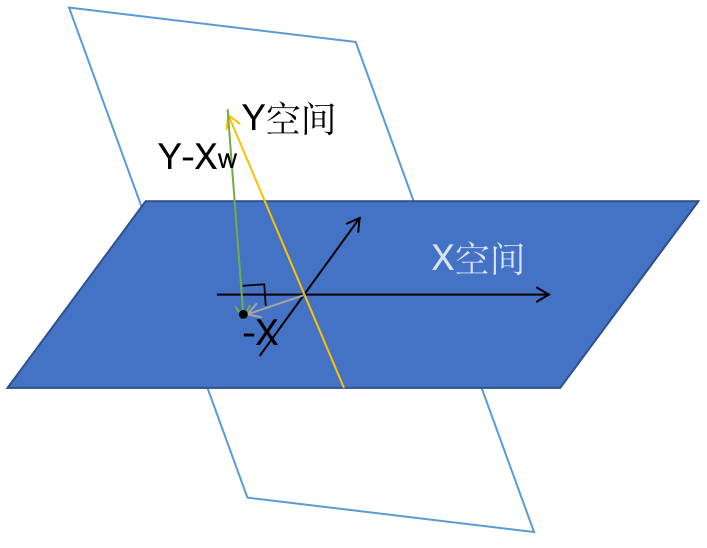
\includegraphics[width=0.7 \textwidth]{/Users/btobab/TeX-Projects/figures/1}
\caption{figure 1}
\end{figure}
Change the model to $f(w)=Xw$, which means zoom $X$ with weight $w$\\\\
The geometric meaning of the least squares method is to find a $w$, so that the distance between vector $Y-Xw$ and space $w$ is the smallest. Of course the case of the smallest distance is perpendicular to space $X$.\\\\
so we get a formula: $X^T(Y-Xw)=0$\\\\
then get the solution of $w$: 
$$
X^TXw=X^TY
$$
$$
\hat{w}=(X^TX)^{-1}X^TY
$$
we can see that the solved $w$ is the same as the result of matrix perspective.
\subsection{Probability perspective}
As we known, in reality, it is hard to fit a distribution with a straight line. True data must have some randomness, that is, noise.\\\\
so we assume noise $\epsilon\backsim N(0,\sigma^2)$\\
so $y=f(w)+\epsilon=w^Tx+\epsilon$\\
so $y|x;w\backsim N(w^Tx,\sigma^2)$\\
Bring it into the probability density function of gaussian distribution:
$$
p(y|x;w)=\frac{1}{\sqrt{2\pi}\sigma}e^{-\frac{(y-w^Tx)^2}{2\sigma^2}}
$$
Then use $MLE$ (maximum likelihood estimate)\\\\
Note: so-called MLE is to get the relative frequency via a large number of samples to approximate probability\\\\
Let's assume a function: $\zeta(w)=\log{p(Y|X;w)}$

Since $n$ data are independent, we can change the probability to a form of continuous mutiplication:

$\zeta(w)=\log{\Pi_{i=1}^np(y_i|x_i;w)}=\Sigma_{i=1}^n \log{p(y_i|x_i;w)}$

bring the probability density function of gaussian distribution into the formula:

$\zeta(w)=\Sigma_{i=1}^n(\log{\frac{1}{\sqrt{2\pi}\sigma}}-\frac{(y-w^Tx)^2}{2\sigma^2})$

since the former term has nothing to do with $w$, it can be ignored.

so:
$$
\hat{w}=argmax{\zeta(w)}
$$
$$
=argmax{ \Sigma_{i=1}^n -\frac{(y-w^Tx)^2}{2\sigma^2}}
$$
$$
=argmin{ \Sigma_{i=1}^n (y-w^Tx)^2}
$$
The conclusion obtained by using maximum likelihood estimation is the definition of least squares method.\\\\
This also shows that least squares method hides a assumption that noise is gaussian distribution.
\newpage
\section{Implement without regularization}
\begin{lstlisting}[language={python}]
%matplotlib inline
import numpy as np
import matplotlib.pyplot as plt

# num of samples
n = 1000
# noise
epsilon = 1
X = np.expand_dims(np.linspace(0,100,1000), axis=-1)
w = np.asarray([5.2])
Y = X  w
# apply noise to X
X += np.random.normal(scale=epsilon, size=(X.shape))
X_T = X.transpose()
w_hat = np.matmul(np.linalg.pinv((np.matmul(X_T, X))), np.matmul(X_T, Y))
print(w_hat)
plt.scatter(X, Y, s=3, c="y")
Y_hat = X  w_hat
plt.plot(X, Y_hat)
plt.show()
\end{lstlisting}
\section{Algorithm with regularization}
\subsection{Matrix perspective}
Firstly, given a new loss functioin with regularization:
$$
\zeta(w)=\Sigma_{i=1}^{n}||y_i-w^T  x_i||^2 + \lambda  ||w||^2
$$
then the derivation of loss function from matrix perspective without regularization is referenced:
$$
\zeta(w)=Y^TY-2w^TX^TY+w^TX^TX w+\lambda  ||w||^2
$$
so$\hat{w}=argmax(\zeta(w))$\\\\
differentiate $\zeta(w)$:
$$
\frac{\partial \zeta(w)}{\partial w}=2X^TXw-2X^T Y+2\lambda  w 
$$
set the derivative equal to 0 to get the closed-form solution of least squares method with regularization:
$$
\hat{w}=(X^TX+\lambda  I)^{-1} X^TY
$$
$I$ is identity matrix
\subsection{Probability perspective}
assume noise $\epsilon \backsim N(0,\sigma_1^2) \ w \backsim N(0,\sigma_2^2)$

since $y=w^T x + \epsilon$

we get $y|w \backsim N(w^T x,\sigma_1^2)$
\\Next we use MAP(Maximum a posteriori estimate):

according to Bayes theorem:
$$
P(w|Y)=\frac{P(Y|w) P(w)}{P(Y)}
$$
$P(w)$ is a priori probability, $P(Y|w)$ is a likelihood probability, $P(Y)$ is normalized probability, priori probability is mutiplied by the likelihood probability and normalized to obtain the posteriori probability $P(w|Y)$.
actually $P(Y)$ is constant, so:
$$
\hat{w}=argmax(P(w|Y))=argmax(P(Y|w) P(w))=argmax(log(P(Y|w) P(w)))
$$
since samples are independent, we can change the probability to a form of continuous mutipication.
$$
=argmax(log(\prod_{i=1}^n P(y_i|w) P(w)))=argmax(\sum_{i=1}^n log(P(y_i|w)+ log(P(w))))
$$
bring it into probability density function of gaussian distribution to get:
$$
\hat{w}=argmax(\sum_{i=1}^nlog(\frac{1}{\sqrt{2\pi} \sigma_1})-\frac{(y_i-w^T x_i)^2}{2\sigma_1^2}+log(\frac{1}{\sqrt{2 \pi} \sigma_2})-\frac{w^2}{2\sigma_2^2})
$$
since both $\sigma_1$ and $\sigma_2$ are hyperparameters, they can be omitted.

so:
$$
\hat{w}=argmin(\sum_{i=1}^n \frac{(y_i-w^T x_i)^2}{2\sigma_1^2}+\frac{w^2}{2\sigma_2^2})
$$
$$
=argmin(\sum_{i=1}^n (y_i-w^T x_i)^2+\frac{\sigma_1^2}{\sigma_2^2} w^2)
$$
we can see that the result derived via $MAP$ is the definition of the least squares method with regularization.
\newpage
\section{Implement with regularization}
\begin{lstlisting}[language={python}]
import os
os.chdir("../")
from models.linear_models import LinearRegression
import numpy as np
import matplotlib.pyplot as plt
X_ = np.expand_dims(np.linspace(0, 10, 1000), axis=-1)
X = np.c_[X_, np.ones(1000)]
w = np.asarray([5.2, 1])
Y = X.dot(w)
X = np.r_[X, np.asarray([[11, 1], [12, 1], [13, 1]])]
Y = np.r_[Y, np.asarray([100, 110, 120])]

model = LinearRegression(l2_ratio=1e1, epoch_num=1000, lr=1e-2, batch_size=100, if_standard=False)
model.fit(X[:, :-1], Y)
print(model.get_params())
model.draw(X[:, :-1], Y)
\end{lstlisting}
\end{document}
\documentclass{report}
\usepackage{amsmath}
\usepackage{amssymb}
\usepackage{listings}
\begin{document}
\section{Perceptron}
\subsection{Abstract}
As we know, linear classificaton is divided into two types:
\begin{itemize}
	\item hard output (directly output the class of the samples):
	\begin{itemize}
		\item perceptron
		\item LDA(linear discriminant analysis)
	\end{itemize}
	\item soft output(output the probability that samples belong to some class):
	\begin{itemize}
	\item gaussian discriminant analysis
	\item logistic regression
	\end{itemize}
\end{itemize}
In this chapter, we will introduce a simple linear binary classification model: Perceptron. Its requirements are relatively loose, as long as we can find a hyperplane to separate positive and negative samples.
\subsection{Idea}
\subsubsection{Error driven}
Literally, we can see that the idea of the perceptron model is to randomly initialize the parameters of the model, and then update its own parameters via errors according to whether the current parameters can correctly separate the positive and negative samples.
\subsection{Algorithm}
Firstly, given the object function of the model:
$$
f(x)=sign(w^Tx)
$$
In this formula, $sign$ is a symbolic function.
$$
sign(a)=
\begin{cases}
+1,\,\,a>0\\
-1,\,\,a\le0\\
\end{cases}
$$
then, according to the idea of perceptron mentioned above: error driven\\
It's easy to obtain the loss function of the model:
$$
L(w)=\sum_{i=1}^n I\{w^Tx_iy_i<0 \}
$$
In this formula, $I$ is a indicator function, indicating which elements belong to the collection.\\
And it's easy to understand the judgment conditions. We note that:
\begin{itemize}
	\item when $y_i>0$, it indicates $y_i$ is a positive sample:
	\begin{itemize}
	\item then, if $w^Tx_i<0$, it indicates the sample is classified incorrectly ($w^Tx_i y_i<0$)
	\item if $w^Tx_i>0$, it indicates the sample is classified correctly ($w^Tx_i y_i>0$)
	\end{itemize} 
	\item when $y_i<0$, it indicates $y_i$ is a negative sample:
	\begin{itemize}
	\item then, if $w^Tx_i<0$, it indicates the sample is classified correctly ($w^Tx_i y_i>0$)
	\item if $w^Tx_i>0$, it indicates the sample is classified incorrectly ($w^Tx_i y_i<0$)
	\end{itemize}
\end{itemize}
We finally find out when $w^Tx_i y_i<0$, it indicates the sample is classified incorrectly by model.
Well, let's look back on the loss function. We are suprised to find that it's non differentiable, thus we can't use gradient descent. Um, how can we solve the issue?\\
We could loose the conditions, and the loss function is updated to:
$$
L(w)=\sum_{(x_i,y_i)\in M} -w^Tx_i y_i
$$
$M$ represents the collection classified incorrectly.\\\\
Then adding a minus sign in front of $w^Tx_i y_i$, we will obtain a positive loss value. And then we can use graident descent to update the parameters $w$.\\\\
As for the derivative of the loss function, it's also easy to solve:

$$
\frac{dL(w)}{dw}=\sum_{(x_i,y_i)\in M} -x_i y_i
$$
\newpage
\subsection{Implement}
\begin{lstlisting}[language={python}]
%matplotlib inline
import os
os.chdir("../")
import numpy as np
from models.linear_models import Perceptron

model = Perceptron(10000, lr=1e-2)
x = np.linspace(0, 100, num=100)
w1, b1 = 0.1, 5
w2, b2 = 0.2, 10
epsilon = 2
k = 0.15
b = 8
w = np.asarray([-k, 1])
v1 = x * w1 + b1 + np.random.normal(scale=epsilon, size=x.shape)
v2 = x * w2 + b2 + np.random.normal(scale=epsilon, size=x.shape)
x1 = np.c_[x, v1]
x2 = np.c_[x, v2]
x = np.r_[x1, x2]
y = np.sign(x.dot(w) - b)
model.fit(x, y)
model.draw(x)
\end{lstlisting}
\end{document}
\documentclass{report}
\usepackage{amsmath}
\usepackage{amssymb}
\usepackage{listings}
\begin{document}
\section{LDA}
\subsection{Abstract}
In this chapter, we will learn another algorithm of the binary-classification-hard-output: LDA (linear discriminant analysis). Actually, it's also used to reduce the dimension.\\\\
We'll select a direction and project the high-dimensional samples to this direction to divide them into two classes.
\subsection{Idea}
The core idea of $LDA$ is to make the projected data satisfy two conditions:
\begin{itemize}
	\item the distance between samples within the same class is close
	\item the distance between different classes is large.
\end{itemize}
\subsection{Algorithm}
Firstly, to reduce the dimension, we have to find out how to calculate the projection length.\\
we assume a sample $x$ and project it to the direction $w$.\\
As we know: $w\cdot x=||w||\ ||x||\ \cos{\theta}$\\\\
Here we assume $||w||=1$ to detemine the unique $w$ to prevent countless solutions caused by scaling.\\
so $w x=||x||\cos{\theta}$\\
And $||x||\cos{\theta}$ is exactly the definition of projection.\\
Therefore, the projection length of the sample on the vector $w$ is $wx$.\\\\
Thus the projection is $z=w^T x$
We assume the number of samples belonging to the two classes is $N1$,$N2$.\\\\
Below, as to the first condition: the distance of sample within the same class is close, we use the variance matrix to represent the overall distribution of each class.\\
Here we use the definitioin of covariance matrix and the covariance matrix of origin data $x$ is denoted as $S$.\\
\begin{equation}
\begin{aligned}C_1: Var_z[C_1]&=\frac{1}{N_1}\sum_{i=1}^{N_1} (z_i-\bar{z_{c1}})(z_i-\bar{z_{c1}})^T\\
&=\frac{1}{N_1}\sum_{i=1}^{N_1}(w^T x_i-\frac{1}{N_1}\sum_{j=1}^{N_1}w^T x_j)(w^T x_i-\frac{1}{N_1}\sum_{j=1}^{N_1}w^T x_j)^T \\&=w^T \frac{1}{N_1}\sum_{i=1}^{N_1}(x_i-\frac{1}{N_1}\sum_{j=1}^{N_1} x_j)(x_i-\frac{1}{N_1}\sum_{j=1}^{N_1} x_j)^T w\\&=w^{T} \frac{1}{N_{1}} \sum_{i=1}^{N_{1}}\left(x_{i}-\bar{x_{c 1}}\right)\left(x_{i}-\bar{x_{c 1}}\right)^{T} w\\&=w^T S_1 w\\C_2: Var_z[C_2]&=\frac{1}{N_2}\sum_{i=1}^{N_2} (z_i-\bar{z_{c2}})(z_i-\bar{z_{c2}})^T\\&=w^T S_2 w
\end{aligned}
\end{equation}
Therefore the distance between classes can be denoted by:
$$
Var_z[C_1]+Var_z[C_2]=w^T(S_1+S_2)w
$$
As to the second condition: the distance between different classes is large\\
The distance between classes can be denoted by the difference between the mean projection length of two classes.
\begin{equation}
\begin{aligned}
(z_{c1}-z_{c2})^2&=(\frac{1}{N_1}\sum_{i=1}^{N_1}w^T x_i - \frac{1}{N_2}\sum_{i=1}^{N_2}w^T x_i)^2\\
&=(w^T(\frac{1}{N_1}\sum_{i=1}^{N_1} x_i - \frac{1}{N_2}\sum_{i=1}^{N_2} x_i))^2\\
&=(w^T(\bar{x_{c1}}-\bar{x_{c2}}))^2\\
&=w^T(\bar{x_{c1}}-\bar{x_{c2}})(\bar{x_{c1}}-\bar{x_{c2}})^T w
\end{aligned}
\end{equation}
Well, let's look back on our two conditions:
\begin{itemize}
	\item the distance of samples within the same class is close
	\item the distance between different classes is large
\end{itemize}
So it's easy to obtain a intuitive loss function:
\begin{equation}
L(w)=\frac{Var_z[C_1]+Var_z[C_2]}{(z_{c1}-z_{c2})^2}
\end{equation}
Via minimizing the loss function, we can obtain the target $w$:
\begin{equation}
\begin{aligned}
\hat{w}=argmin(L(w))&=argmin(\frac{Var_z[C_1]+Var_z[C_2]}{(z_{c1}-z_{c2})^2})\\
&=argmin(\frac{w^T(S_1+S_2)w}{w^T(\bar{x_{c1}}-\bar{x_{c2}})(\bar{x_{c1}}-\bar{x_{c2}})^T w})\\
&=argmin(\frac{w^T S_w w}{w^T S_b w})\\
\end{aligned}\end{equation}
In the formula:
\begin{equation}
\begin{aligned}
&S_w: with-class:variance\ within\ the\ class\\
&S_b: between-class:variance\ between\ classes\\
\end{aligned}
\end{equation}
The following is the partial derivative of the above formula:\\
\begin{equation}
\begin{aligned}
\frac{\partial{L(w)}}{\partial{w}}
&=\frac{\partial}{\partial{w}}(w^T S_w w)(w^T S_b w)^{-1}\\
&=2S_{b} w\left(w^{T} S_{w} w\right)^{-1}-2 w^{T} S_{b} w\left(w^{T} S_{w} w\right)^{-2} S_{w} w=0\\
\end{aligned} \end{equation}
try to transform the equation:
$$
\begin{aligned}
\left(w^{T} S_{b} w\right) S_{w} w&=S_{b} w\left(w^{T} S_{w} w\right)\\
\left(w^{T} S_{b} w\right) w&=S_{w}^{-1}S_{b} w\left(w^{T} S_{w} w\right)
\end{aligned}
$$
Notes: the shape of $w^T S_b w$ and $w^T S_w w$ is : $(1,p)(p,p) (p,1)=(1,1)$\\\\
Since the two terms are scalars, they only scale the module of a vector and can't change its direction, so the above formula is updated to:
$$
w \propto S_{w}^{-1} S_{b} w=S_{w}^{-1}\left(\bar{x_{c 1}}-\bar{x_{c 2}}\right)\left(\bar{x_{c 1}}-\bar{x_{c 2}}\right)^{T} w 
$$
And because $\left(\bar{x_{c 1}}-\bar{x_{c 2}}\right)^{T} w$ is also a scalae, we obtain the final formula:
$$
\hat{w}\propto S_{w}^{-1}\left(\bar{x_{c 1}}-\bar{x_{c 2}}\right)
$$
So $S_{w}^{-1}\left(\bar{x_{c 1}}-\bar{x_{c 2}}\right)$ is the direction we have been seeking, finally we can get the standard $w$ via scaling.
\newpage
\subsection{Implement}
\begin{lstlisting}[language={python}]
import numpy as np
import os
os.chdir("../")
from models.linear_models import LDA

x = np.linspace(0, 100, num=100)
w1, b1 = 0.1, 10
w2, b2 = 0.3, 30
epsilon = 2
k = 0.2
b = 20
w = np.asarray([-k, 1])
v1 = x * w1 + b1 + np.random.normal(scale=epsilon, size=x.shape)
v2 = x * w2 + b2 + np.random.normal(scale=epsilon, size=x.shape)
x1 = np.c_[x, v1]
x2 = np.c_[x, v2]
l1 = np.ones(x1.shape[0])
l2 = np.zeros(x2.shape[0])
data = np.r_[x1, x2]
label = np.r_[l1, l2]

model = LDA()
model.fit(x1, x2)
model.draw(data, label)
\end{lstlisting}
\end{document}
\documentclass{report}
\usepackage{amsmath}
\usepackage{amssymb}
\usepackage{listings}
\begin{document}
\chapter{Logistic Regression}
\section{Abstract}
In this chapter, we will learn an algorithm for binary classification - soft output: Logistic regression. It mainly relies on an activation function: $sigmoid$. Since the range of the function is $(0,1)$, it can approximate the probability value.
\section{Origin}
The following is the explanation of sigmoid in $shuhuai$ teacher's handout.
\begin{quotation}
	Sometimes we only need to get the probability of a category, so we need a function that can output the value of $(0, 1)$ interval. Considering the two classification model, we hope to model $p(C|x)$ using the discriminant model and Bayesian theorem: $$p\left(C_{1} \mid x\right)=\frac{p\left(x \mid C_{1}\right) p\left(C_{1}\right)}{p\left(x \mid C_{1}\right) p\left(C_{1}\right)+p\left(x \mid C_{2}\right) p\left(C_{2}\right)}$$
\end{quotation}
set $a=\ln \frac{p\left(x \mid C_{1}\right) p\left(C_{1}\right)}{p\left(x \mid C_{2}\right) p\left(C_{2}\right)}$, so:
$$
p\left(C_{1} \mid x\right)=\frac{1}{1+\exp (-a)}
$$
The above formula is called $Logistic\ Sigmoid$ function and its parameters denote the logarithm of the two types of the joint probability ratios. In the discriminant, we don't care the specific value of the parameter and we just use the form of the function.\\\\
Of course, it doesn't matter if we can't understand tearcher's advanced explanation. We just need to know that we have the activation function $sigmoid$ now, which can be used to get the probability of a category.
\section{Algorithm}
Firstly, we suppose the logistic regression model is:
$$
f(x)=\sigma(w^Tx)
$$
In the formula, $\sigma(a)=sigmoid(a)$, we usually denote the activation function by $\sigma$.\\
So, if we find out the best value of $w$, the best model under the assumption is determined.\\
The parameters of probability discrinant model is usually determined by maximum likelihood estimation.\\
To determine the likelihood function, we have to make some marks firstly:
$$
p_1=\sigma(w^Tx) \qquad p_0=1-p_1
$$
In the formula, $p_1$ is the probability of $x$ belonging to class $1$ and $p_0$ is the probability of class $0$.\\
Then we can obtain the likelihood function of the model:
$$
p(y|w;x)=p_1^yp_0^{1-y}
$$
The likelihood function seem to be a little obscure, but actually it's reasonable:
\begin{itemize}
	\item when $y$ is $1$: $p(y|w;x)=p_1^1p_0^0=p_1$
	\item when $y$ is $0$: $p(y|w;x)=p_1^0p_0^1=p_0$
\end{itemize}
Well, then we can determine the parameters via $MLE$.
\begin{equation}
\begin{aligned}
\hat{w}=argmax(J(w))&=argmax(p(Y|w;X))\\
&=argmax(log(p(Y|w;X)))\\
&=argmax(log(\prod_{i=1}^n p(y_i|w;x_i)))\\
&=argmax(\sum_{i=1}^n log(p(y_i)|w;x_i))\\
&=argmax(\sum_{i=1}^n y\ log\, p_1+(1-y)log\,p_0)
\end{aligned}
\end{equation}
Notes, the formula is the opposite of the cross entropy formula mutiplied by $N$ and the logarithm in $MLE$ also match the exponential function to obtain the stable gradient in a large interval.\\\\
By differentiating the above formula, we note that:
$$
p_1'=p_1(1-p_1)
$$
Of course, it's easy to obtain since it's just the chain rule. We only need to be a little bit careful.\\
Finally, we obtain the result:
$$
\frac{\partial}{\partial w}J(w)=\sum_{i=1}^{N}\left(y_{i}-p_{1}\right) x_{i}
$$
Last but not least, we are to obtain the maximun of $p(p|w;x)$, so we need to use gradient ascent instead of gradient descent. Certainly they are similar, just add a negative character.
\section{Implement}
\begin{lstlisting}[language={python}]
import os
os.chdir("../")
from models.linear_models import Logistic_regression
import numpy as np
import warnings

epsilon = 1
num_test = 100
num_base = 1000
ratio = 0.6
k1, k2 = 3, 5
b1, b2 = 1, 2
X = np.linspace(0, 100, num_base)
X_train = X[:-num_test]
X_test = X[-num_test:]
v1 = X_train[:round(len(X_train) * ratio)] * k1 + b1
v2 = X_train[round(len(X_train) * ratio):] * k2 + b2
v1 += np.random.normal(scale=epsilon, size=v1.shape)
v2 += np.random.normal(scale=epsilon, size=v2.shape)
value = np.r_[v1, v2]
data = np.c_[X_train, value]
l1 = np.ones_like(v1)
l2 = np.zeros_like(v2)
label = np.r_[l1, l2]
v_test_c1 = X_test * k1 + b1
l_test_c1 = np.ones_like(v_test_c1)
data_test = np.c_[X_test, v_test_c1]

model = Logistic_regression(10, 1000, lr=1e-3)
model.fit(data, label)
print(model.get_params())
print(model.predict(data_test, l_test_c1))
\end{lstlisting}
\end{document}
\documentclass{report}
\usepackage{amsmath}
\usepackage{amssymb}
\usepackage{listings}
\begin{document}
\section{GDA}
\subsection{Abstract}
In this chapter, we will learn an algorithm of linear classification - soft output - probability generation model: GDA (Gaussian Discriminant Analysis).
\subsection{Idea}
In the last chapter, the logistic regression algorithm we learned belongs to probability discriminant model, so the difference between the discriminant model and the generation model is:
\begin{itemize}
	\item the discriminant model is used to model the probability $p(y|x)$ directly to obtain its truly probability value.
	\item the generation model is used to model the joint distribution $(x,y)$ via converting $p(y|x)$ to $p(x|y)p(y)$ according to bayes theorem: $p(y|x)=\frac{p(x|y)p(y)}{p(x)}$. Since $p(x)$ has nothing to do with $y$, it can be omitted. So, finally we get:$$
p(y|x)\propto p(x|y)p(y)=p(x;y)
$$
\end{itemize}
when we are to predict any samples, we just need to compare $p(y=0|x)$ and $p(y=1|x)$.
\subsection{Algorithm}
Firstly, let's make some assumption about the model:
$$
y\in \{0,1\}\quad y\sim Bernuolli(\phi)\quad p(y)=\phi^y(1-\phi)^{1-y}\\\left \{\begin{aligned}x|y=1 \quad \sim \quad N(\mu_1,\Sigma)\\x|y=0 \quad \sim \quad N(\mu_2,\Sigma)\end{aligned}\right.
$$
$$
\Longrightarrow p(x|y)=N(\mu_1,\Sigma)^yN(\mu_2,\Sigma)^{1-y}
$$
so all the parameters $\theta$ of the model are:
$$
\theta=(\phi, \mu_1, \mu_2, \Sigma)
$$
Then given the loss function of the model:
$$
\begin{aligned}
J(\theta)=log(p(Y|X))&=log(\prod_{i=1}^n p(y_i|x_i))\\
&=\sum_{i=1}^n log(p(y_i|x_i))\\
\end{aligned}
$$
so:
$$
\begin{aligned}
\hat{\theta}=argmax(J(\theta))&=argmax(\sum_{i=1}^nlog(\frac{p(x_i|y_i)p(y_i)}{p(x_i)}))\\
&=argmax(\sum_{i=1}^n log(p(x_i|y_i)p(y_i)))\\
&=argmax(\sum_{i=1}^n y_i\ log(N(\mu_1,\Sigma))+(1-y_i)\ log(N(\mu_2,\Sigma))+log(\phi^{y_i} (1-\phi)^{1-y_i}))
\end{aligned}
$$
\subsubsection{Solve $\phi$}
differentiate $\phi$:
$$
\sum_{i=1}^{N} \frac{y_{i}}{\phi}+\frac{y_{i}-1}{1-\phi}=0
\Longrightarrow \phi=\frac{\sum_{i=1}^{N} y_{i}}{N}=\frac{N_{1}}{N}
$$
In the formula, $N,N_1,N_2$ denote the number of all samples, positive samples, negative samples.
\subsubsection{Solve $\mu$}
make some derivations based on $J(\theta)$:
$$
\begin{aligned} \hat{\mu_{1}} 
&=\underset{\mu_{1}}{argmax} \sum_{i=1}^{N} y_{i} \log N\left(\mu_{1}, \Sigma\right) \\
&=\underset{\mu_1}{argmax} \sum_{i=1}^{N} y_i \log (\frac{1}{(2\pi)^{\frac{p}{2}}|\Sigma|^{\frac{1}{2}}}exp(-\frac{1}{2}(x_i-\mu_1)^T(\Sigma)^{-1}(x_i-\mu_1)))\\
&=\underset{\mu_{1}}{argmin} \sum_{i=1}^{N} y_{i}\left(x_{i}-\mu_{1}\right)^{T} \Sigma^{-1}\left(x_{i}-\mu_{1}\right)
\end{aligned}
$$
In the above derivations, we quote the probability density function of multivariate Gaussian distribution:
$$
p(x)=\frac{1}{(2\pi)^{\frac{p}{2}}|\Sigma|^{\frac{1}{2}}}exp(-\frac{1}{2}(x_i-\mu_1)^T(\Sigma)^{-1}(x_i-\mu_1))
$$
In the function, $p$ denote the number of random variables. Readers can multiply the probability density function of univariate Gaussian distribution, and derive the multivariate formula with the knowledge of linear algebra.\\
then differentiate the formula:
$$
\frac{\partial \Delta}{\partial \mu_1}=\sum_{i=1}^N -2y_i (\Sigma)^{-1}(x_i-\mu_1)=0\\
\Longrightarrow \mu_{1}=\frac{\sum_{i=1}^{N} y_{i} x_{i}}{\sum_{i=1}^{N} y_{i}}=\frac{\sum_{i=1}^{N} y_{i} x_{i}}{N_{1}}
$$
Since the positive samples and the negative samples are symmetrical, therefore:
$$
\mu_{2}=\frac{\sum_{i=1}^{N}\left(1-y_{i}\right) x_{i}}{N_{2}}
$$
\subsubsection{Solve $\Sigma$}
observe the first two terms of the formula:
$$
\hat{\theta}=argmax(\sum_{i=1}^n y_i\ log(N(\mu_1,\Sigma))+(1-y_i)\ log(N(\mu_2,\Sigma))+log(\phi^{y_i} (1-\phi)^{1-y_i}))
$$
We note that when $y=0$, the first term equals to $0$; when $y=1$, the second term equals to $0$.\\
thus the formula can be updated to:
$$
\begin{aligned}
\hat{\theta}
&=argmax(\sum_{(x_i,y_i)\in C_1} \ log(N(\mu_1,\Sigma))+\sum_{(x_i,y_i)\in C_2}\ log(N(\mu_2,\Sigma)))\\
&=argmax(\sum_{(x_i,y_i)\in C_1} -\frac{1}{2}\log|\Sigma|-\frac{1}{2}(x_i-\mu_1)^T(\Sigma)^{-1}(x_i-\mu_1)\ +\\
&\sum_{(x_i,y_i)\in C_2} -\frac{1}{2}|\Sigma|-\frac{1}{2}(x_i-\mu_2)^T(\Sigma)^{-1}(x_i-\mu_2))
\end{aligned}
$$
Note the shape of $(x_i-\mu)^T(\Sigma)^{-1}(x_i-\mu)$ : $(1,p)* (p,p) * (p,1)=(1,1)$, therefore, the trace(tr) operation can be applied to it, and it can be regarded as a matrix. Within the trace, the order of matrices can be exchanged at will.
$$
\begin{aligned}
\hat{\theta}
&=argmax(-\frac{N}{2}\log|\Sigma|-\frac{1}{2}tr(\sum_{(x_i,y_i)\in C_1}(x_i-\mu_1)^T(\Sigma)^{-1}(x_i-\mu_1))\\
&-\frac{1}{2}tr(\sum_{(x_i,y_i)\in C_2}(x_i-\mu_2)^T(\Sigma)^{-1}(x_i-\mu_2)))\\
&=argmax(-\frac{N}{2}\log|\Sigma|-\frac{1}{2}tr(\sum_{(x_i,y_i)\in C_1}(x_i-\mu_1)^T(x_i-\mu_1)(\Sigma)^{-1})\\
&-\frac{1}{2}tr(\sum_{(x_i,y_i)\in C_2}(x_i-\mu_2)^T(x_i-\mu_2)(\Sigma)^{-1}))\\
&=argmax(-\frac{N}{2}\log|\Sigma|-\frac{1}{2}tr(N_1 S_1(\Sigma)^{-1})
-\frac{1}{2}tr(N_2 S_2(\Sigma)^{-1}))\\
\end{aligned}
$$
In the formula, $S$ denote the co-variance matrix.\\
differentiate the formula:
$$
\frac{\partial \Delta}{\partial \Sigma}=-\frac{1}{2}(N \frac{1}{|\Sigma|}|\Sigma|(\Sigma)^{-1}-N_1S_1(\Sigma)^{-2}-N_2S_2(\Sigma)^{-2})=0
$$
then we obtain the $\hat{\Sigma}$: 
$$
N \Sigma^{-1}-N_{1} S_{1}^{T} \Sigma^{-2}-N_{2} S_{2}^{T} \Sigma^{-2}=0\\
\Longrightarrow \hat{\Sigma}=\frac{N_{1} S_{1}+N_{2} S_{2}}{N}
$$
Finally, when we are to predict any samples, we just need to compare $p(x|y=0)p(y=0)$ and $p(x|y=1)p(y=1)$.
\subsection{Implement}
\begin{lstlisting}[language={python}]
import numpy as np
import os
os.chdir("../")
from models.linear_models import GDA

n1 = 1000
n_test = 100
x = np.linspace(0, 10, n1 + n_test)
w1, w2 = 0.3, 0.5
b1, b2 = 0.1, 0.2
x1 = x[:n1]
x_test = x[n1:]
v1 = x1 * w1 + b1
v2 = x1 * w2 + b2
cla_1 = np.c_[x1, v1]
cla_2 = np.c_[x1, v2]
l1 = np.ones(shape=(cla_1.shape[0], 1))
l2 = np.zeros(shape=(cla_2.shape[0], 1))
train_data = np.r_[cla_1, cla_2]
train_label = np.r_[l1, l2]

v_test = x_test * w2 + b2
data_test = np.c_[x_test, v_test]

model = GDA()
model.fit(train_data, train_label)
print(model.get_params())
print("accuary:", model.evaluate(data_test, 0))
\end{lstlisting}
\end{document}
\documentclass{report}
\usepackage{amsmath}
\usepackage{amssymb}
\usepackage{listings}
\begin{document}
\section{Naive bayes Classify}
\subsection{Abstract}
In this issue, we will learn an another algorithm linear classification - soft output - probability generation model: Naive Bayes Hypothesis.
\subsection{Idea}
In the last issue, GDA we learned makes an assumption that the dataset obeys Gaussian Dist. At the same time, Bernoulli Dist is introduced as a priori of the label to obtain the parameters via MAP.\\\\
Naive bayes Hypothesis we learned in this issue assumes the relationship between the attributes of the data: the conditional independence hypothesis.
\subsection{Algorithm}
Normally, since there is $p$ dimensions in $x$, we need to sample the joint distribution of $p$ random variables to get the probability $p(x|y)$. However, as we know: A huge number of samples are needed to obtain the relative accurate probability approximation as to the high-dimensional space.\\\\
In the general directed probability graph model, different assumptions are made on the conditional independence relationship between various attribute dimensions, among which the simplest assumption is that one described in Naive Bayes model:
$$
p(x|y)=\prod_{i=1}^p p(x_i|y)p(y)
$$
In mathematical language:
$$
x_{i} \perp x_{j} | y, \forall i \neq j
$$
for a simple observation with Bayesian theorem:
$$
p(y|x)=\frac{p(x|y)p(y)}{p(x)}=\frac{\prod_{i=1}^p p(x_i|y)p(y)}{p(x)}
$$
Similar to GDA, here are some assumptions about the distributions of the data:
\begin{itemize}
	\item $x_i$ is a discrete variable:
	\begin{itemize}
	\item Generally, we assume $x_i$ obey Categorical Dist: $p(x_i=i|y)=\theta_i,\sum_{i=1}^p \theta_i =1$
	\end{itemize}
	\item $x_i$ is a continuous variable:
	\begin{itemize}
	\item Generally, we assume $x_i$ obey Gaussian Dist: $p(x_i|y)=N(\mu_i, \Sigma_i)$
	\end{itemize}
\end{itemize}
\begin{itemize}
	\item Binary classification:
	\begin{itemize}
	\item $y \backsim Bernoulli(\phi):p(y)=\phi^y (1-\phi)^{(1-y)}$ 
	\end{itemize}
	\item Multi-classification:
	\begin{itemize}
	\item $y \backsim Categorical\ Dist\quad p(y_i)=\theta_i\quad \sum_{i=1}^k \theta_i=1$
	\end{itemize}
\end{itemize}
We are used to sample the dataset to estimate the parameters. we'll obtain the posteriori probability with Bayesian theorem when we are to predict test data after estimating the parameters.
\subsection{Implement}
\begin{lstlisting}[language={python}]
import numpy as np
import os
os.chdir("../")
from models.linear_models import NaiveBayesClassifier

num_test = 100
x = np.linspace(0, 10, 1000)
k1, k2 = 0.1, 0.3
b1, b2 = 1, 2
x_train = x[:-num_test]
x_test = x[-num_test:]
v_1 = x_train * k1 + b1
v_2 = x_train * k2 + b2
train_data = np.r_[np.c_[x_train, v_1], np.c_[x_train, v_2]]
train_label = np.r_[np.ones_like(x_train), np.zeros_like(x_train)]

model = NaiveBayesClassifier()
model.fit(train_data, train_label)
print(model.get_params())

v_test = x_test * k2 + b2
data_test = np.c_[x_test, v_test]
print("accuary:", model.predict(data_test, 0))
\end{lstlisting}
\end{document}
\documentclass{report}
\usepackage{amsmath}
\usepackage{amssymb}
\usepackage{listings}
\begin{document}
\section{PCA}
\subsection{Abstract}
In this issue, we begin to learn the algorithm of dimension reduction.\\\\
As we know, dimension reduction is the best way to solve the problem of over fitting, in addition to increasing data and regularization.\\\\
In fact, the predecessors had encountered dimensional disasters earlier. We know that the volume of the $n $ dimensional sphere is $CR^n$\\\\
Therefore, the ratio of the volume of the sphere to the $n$ dimensional hypercube is
$$
\lim_{n \to +\infty}=\frac{CR^n}{2^n R^n}=0
$$
From the formula, we can see that in high-dimensional data, the distribution of samples is quite sparse, and the interior of hypercube is almost hollow, so it is more difficult to model the data. This is the so-called dimensional disaster.

The dimensionality reduction methods are divided into:
\begin{itemize}
	\item Direct dimensionality reduction, feature selection
	\item Linear dimensionality reduction, PCA, MDS etc.
	\item Piecewise linear, manifolds include Isomap, LLE etc.
\end{itemize}
\subsection{Idea}
As for the core idea of PCA, the teacher summarized a line: one center, two basic points
\begin{itemize}
	\item one center:
	\begin{itemize}
	\item to transform each feature that may be linearly related into a set of linearly independent features via an orthogonal transformation.
	\item That is, to reconstruct the original feature space.
	\end{itemize}
	\item Two basic points:
	\begin{itemize}
	\item Maximum Projection Variance
	\begin{itemize}
	\item Make the data more dispersed in the reconstructed feature space (because the original data is clustered together and scattered in corners)
	\end{itemize}
	\item Minimum Reconfiguration Distance
	\begin{itemize}
	\item to minimize the loss of information (i.e., fewer components of the complementary space) after the data has been reconstructed
	\end{itemize}
	\end{itemize}
\end{itemize}
\subsection{Algorithm}
we'll mainly talk about the first basic point: maximum projection variance. In fact, the two basic points mean the same thing, but interpret a center from different angles.\\\\
Firstly,we are to review the projection. We have talked about projection before, and the same is true here. Let's assume sample $x_ i $, a base vector $u_ i $, assuming $u_ i^Tu_ i = 1 $, so you can get the projection of the sample in  this dimension $u_ i $ is
$$
project_i=x_i^Tu_i
$$
After orthogonal transformation, the sample originally has $p $ feature dimensions. Because we need to reduce the dimension, we only take the first $q $ features, and these $q $ features are linearly independent. Therefore, these projections can be directly added to obtain the projection of the sample in the new feature space.\\\\
Note that the data is centered before the projection, so the mean value of the data is changed to zero, and the variance of the projection can be squared directly.\\
To sum up, we get the objective function:
$$
J=\frac{1}{N} \sum_{i=1}^{N} \sum_{j=1}^{q}\left(\left(x_{i}-\bar{x}\right)^{T} u_{j}\right)^{2}
$$
The objective function is derived slightly below:\\
since the shape of $((x_i-\bar{x})^Tu_j)$ is $(1,p)* (p,1)=(1,1)$, therefore, it can be transposed:
$$
\begin{aligned}
J&=\frac{1}{N} \sum_{i=1}^{N} \sum_{j=1}^{q}\left(\left(x_{i}-\bar{x}\right)^{T} u_{j}\right)^{2}\\
&=\frac{1}{N} \sum_{i=1}^{N} \sum_{j=1}^{q}(u_{j}^T(x_{i}-\bar{x}))^{2}\\
&=\frac{1}{N} \sum_{i=1}^{N} \sum_{j=1}^{q}u_{j}^T(x_{i}-\bar{x}))(x_{i}-\bar{x})^T u_j\\
&=\sum_{j=1}^{q} u_{j}^T(\frac{1}{N} \sum_{i=1}^{N} (x_{i}-\bar{x}))(x_{i}-\bar{x})^T) u_j\\
&=\sum_{j=1}^q u_j^T S u_j\\
\end{aligned}
$$
Don't forget that we have another condition: $s.t\ u_j^T u_j=1$\\\\
So you can use Lagrange multiplier:
$$
\underset{u_{j}}{\operatorname{argmax}} L\left(u_{j}, \lambda\right)=\underset{u_{j}}{\operatorname{argmax}} u_{j}^{T} S u_{j}+\lambda\left(1-u_{j}^{T} u_{j}\right)
$$
To derive from the above:
$$
\frac{\partial \Delta}{\partial u_j}=2S u_j -2\lambda u_j=0
$$
we get:
$$
S u_j = \lambda u_j
$$
You can see that the transformed base vector is actually the eigenvector of the covariance matrix, $\lambda$ is the eigenvalue of $S$.\\
In fact, the solution of covariance matrices can also be simplified:
$$
\begin{aligned}
S &=\frac{1}{N} \sum_{i=1}^{N}\left(x_{i}-\bar{x}\right)\left(x_{i}-\bar{x}\right)^{T} \\
&=\frac{1}{N}\left(x_{1}-\bar{x}, x_{2}-\bar{x}, \cdots, x_{N}-\bar{x}\right)\left(x_{1}-\bar{x}, x_{2}-\bar{x}, \cdots, x_{N}-\bar{x}\right)^{T} \\
&=\frac{1}{N}\left(X^{T}-\frac{1}{N} X^{T} I_{N} I_{N}^{T}\right)\left(X^{T}-\frac{1}{N} X^{T} I_{N} I_{N}^{T}\right)^{T} \\
&=\frac{1}{N} X^{T}\left(E_{N}-\frac{1}{N} I_{N} I_{N}^T\right)\left(E_{N}-\frac{1}{N} I_{N} I_{N}^T\right)^{T} X \\
&=\frac{1}{N} X^{T} H_{N} H_{N}^{T} X \\
&=\frac{1}{N} X^{T} H_{N} H_{N} X=\frac{1}{N} X^{T} H X
\end{aligned}
$$
Here, $H$ is a special matrix, called a central matrix.
$$
H=E_N - \frac{1}{N}I_N I_N^T
$$
Therefore, in practice, we only need to find the covariance matrix using the above formula, and then decompose it orthogonally to get the eigenvalues and eigenvectors.
\newpage
\subsection{Implement}
\begin{lstlisting}[language={python}]
import numpy as np
import os
os.chdir("../")
from models.decompose_models import PCA

k, b = 3, 4
x = np.linspace(0, 10, 100)
y = x * k + b
x += np.random.normal(scale=0.3, size=x.shape)
data = np.c_[x, y]

model = PCA()
model.fit(data)
model.draw(data)
\end{lstlisting}
\end{document}
\documentclass{report}
\usepackage{amsmath}
\usepackage{amssymb}
\usepackage{listings}
\begin{document}
\section{PCoA}
\subsection{Abstract}
In the last issue, we learned the derivation process of the formula of PCA, but it is more troublesome in practical use. The co-variance matrix needs to be obtained first, and then apply singular value decomposition to it. \\
Therefore, the more common method is to directly perform singular value decomposition on the centralized data set.\\\\
In addition, using principal component analysis, we finally get a new coordinate base. To reduce the dimension of the data set, we also need to project the coordinates. Therefore, this issue will introduce a similar but simpler method: principal coordinate analysis (PCoA)
\subsection{Algorithm}
\subsubsection{SVD and PCA}
In the previous issue, we derived a simplified form of the co-variance matrix:
$$
S=\frac{1}{N} X^T H X
$$
At the same time, we also derived that the central matrix $H^2\ and\ H^T $are their own $H $.\\\\
Therefore:
$$
S=\frac{1}{N} X^T H^T H X
$$
Because we can perform singular value decomposition on any matrix, we have:
$$
HX = U \Sigma V^T
$$
Therefore, it is substituted into the covariance matrix:
$$
S = V \Sigma U^T U \Sigma V^T
$$
As we all know:
$$
U^T U=I \quad V^T V = V V^T= I \quad \Sigma \ is \ diagonal\ matrix:
$$
Therefore:
$$
S=V\Sigma ^2 V^T
$$
Here, we find that we can get the eigen value $\ sigma $and eigen vector $V $ of the co-variance matrix by singular value decomposition of the centralized data set.\\\\
We calculate $HXV $ to get the projected coordinates.
\subsubsection{PCoA}
Let's reverse the form of $S $ and construct a matrix:
$$
T=HXX^TH^T
$$
Similar to the above process, we get:
$$
\begin{aligned}
T&=HXX^TH^T\\
&=U\Sigma V^T V\Sigma U^T\\
&=U\Sigma^2 U^T
\end{aligned}
$$
We will slightly derive the projected coordinates:
$$
HXV=U\Sigma V^TV=U\Sigma
$$
Therefore, the principal coordinate analysis can directly calculate the projection coordinates
\end{document}
\end{document}}